\documentclass[12pt,a4paper]{report}
\usepackage[latin1]{inputenc}
\usepackage[spanish]{babel} % espanol
\usepackage{amsmath}
\usepackage{amsfonts}
\usepackage{amssymb}
\usepackage{graphicx}
\usepackage{array}
\usepackage[left=2.00cm, right=2.00cm, top=2.00cm, bottom=2.00cm]{geometry}
\author{Julian David Mora Ramos}
\title{Informe de visibilidad}
\begin{document}
	\title{%
		Visibilidad \\
		\large Visualizaci�n web y gesti�n de eventos de los Semilleros de Investigaci�n de la Universidad de la Amazonia \\
		Proyecto ligado al sistema SIGEPI}
	\author{
		Julian David$^{1}$, Valentina Rios$^{2}$, \\ 
		Manuel Hernandez$^{3}$, Mitch Aguilar$^{4}$ \\ 
		W. Emiro Castrill�n $^{5}$ \\ 
		\\
		\small{$^{1-5}$Universidad de la Amazonia, $^{1-5}$Florencia,Caquet�}\\
	}	
	\maketitle
	
	\tableofcontents
	
	\begin{center}
		\chapter*{Visibilidad}
	\end{center}

	\section{Frameworks y sistemas usados}
	
	\begin{itemize}
		\item MVC 5 .NET. Solo Razor
		\item VueJS. Framework de Javascript. Usado para desarrollo de interfaces din�micas.
		\item Oracle. Gestor de bases de datos.
	\end{itemize}
	
	\section{Resumen general}
	
	\begin{center}
		\begin{tabular}{|l|p{3cm}|p{3.5cm}|rc|}
			\hline
			\textbf{Controladores} & \textbf{Vistas} & \textbf{Procedimientos} & \textbf{Estado actual} & \\
			\hline
			42 controladores & 140 vistas aproximadamente & 212 procedimientos almacenados & 90\% del software total & \\
			\hline
		\end{tabular}		
	\end{center}
	
	Por cada procedimiento almacenado existente, hay una funci�n en el controlador.
	En total, hay 212 procedimientos almacenados hasta ahora \textit{(\today)}. Cada procedimiento est� referenciado en una funci�n de los controladores C\#, por lo tanto hay m�s de 212 funciones, esto incluye funciones tipo API (aprox. cuatro controladores) y cerca del 90\% son funciones de renderizaci�n de vistas (Razor).
	
	\section{Resumen de actividades}
	
	\begin{center}
		\begin{tabular}{|l|p{3cm}|l|c|}
					\hline 
					\textbf{Asistente de desarrollo} & \textbf{Aporte en \# lineas (C�digo)} & \textbf{Tareas realizadas} & \textbf{Tiempo} \\					
					\hline 
					
					Valentina R�os & 12.061 lineas & 
						\begin{tabular}{c|p{4cm}}
							&\\						
							1 & Validaci�n de procedimientos almacenados para actualizar, crear, eliminar y ver en detalle. Esto mismo aplicado a los 212 procedimientos almacenados existentes. \\ 
							\hline 
							2 & Creaci�n y arreglo de algunos procedimientos almacenados, tablas, secuencias y disparadores \\ 
							\hline 
							3 & Comprobaci�n y arreglo de vistas Razor. \\
							\hline 
							4 & Correcci�n de algunos m�todos en los controladores. \\
						\end{tabular} 
					& Febrero-Marzo \\ 
					\hline
					
					Maicol Aguilar & 4.166 lineas & 
						\begin{tabular}{c|p{4cm}}
							&\\						
							1 & Creaci�n y mejoramiento de vistas publicas: 'Acerca de', la pagina principal de Visibilidad. \\ 
							\hline 
							2 & Adaptaci�n de algunos formularios al estilo material de Google, \textit{Boostrap material design}. \\ 
							\hline 
							3 & Dise�o de algunas otras interfaces gr�ficas \\
						\end{tabular} 
					& Febrero-Marzo \\ 
					\hline
				
					Manuel Hernandez & 3.018 lineas & 
					\begin{tabular}{c|p{4cm}}
						&\\						
						1 & Comprobaci�n y mejoramiento de vistas. \\ 
						\hline 
						2 & Creaci�n de procedimientos almacenados para eliminaci�n de datos \\
						\hline 
						3 & Comprobaci�n del funcionamiento de algunos procedimientos \\
					\end{tabular}
					& Febrero-Marzo \\ 					
					\hline 
					
					Wilmer Emiro Castrillon & 1.597 lineas & 
					\begin{tabular}{c|p{4cm}}					
						1 & Adaptaci�n de la vista principal (Index) con Google maps. \\ 
						\hline
						2 & Inserci�n de datos de prueba en tablas de la base de datos \\
					\end{tabular}
					& Febrero-Marzo \\
					\hline 					
				\end{tabular} 
	\end{center}

	\begin{figure}
		La imagen a continuaci�n muestra el intervalo de aportes medido por cantidad de lineas de c�digo enviadas. Como se puede notar a continuaci�n, se puede ver que cada asistente ha realizado una cantidad determinada de aportes, pero tambi�n se observa el numero de lineas eliminadas {\small (N�meros en color rojo)}. La altura cada cresta en las gr�fica es proporcional a la cantidad de aportes realizados en un determinado intervalo de tiempo \textit{(meses)}. \\ \\
		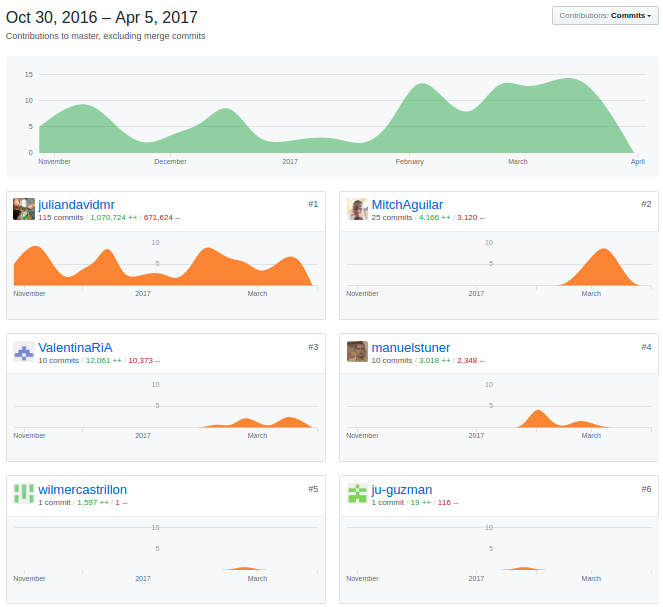
\includegraphics[width=\textwidth]{resources/resumen_github_commits.png}
		\caption{Gr�fica de contribuci�n}
	\end{figure}

	
	\section{Estado actual}
	\begin{tabular}{|p{3cm}|p{6cm}|c|}
		\hline
		\textbf{Caracter�stica} & \textbf{Descripci�n} & \textbf{Funciones disponibles} \\ 
		\hline
		
		Chair� & Inicio de sesi�n usando las credenciales de chair� & 
		\begin{tabular}{cp{4cm}}	
			1 & Registro automatizado \textit{(No es necesario registrarse)}. Se requiere una cuenta de Chaira. \\ 
			\hline 
			2 & Acceso r�pido mediante API \\ 
		\end{tabular} \\ 
		\hline
		
		Noticia & Los lideres de los semilleros y grupos de investigaci�n pueden publicar noticias referentes a su organizaci�n. & 
		\begin{tabular}{lp{4cm}}	
			1 & Visualizaci�n de noticias en una vista general \\ 
			\hline 
			2 & Actualizaci�n de noticias\\ 
			\hline 
			3 & Registro de noticias con intervalo de visualizaci�n. \\
		\end{tabular} \\
		\hline
		
		Actividad & Los lideres de los semilleros y grupos de investigaci�n pueden publicar actividades referentes a su organizaci�n. & 
		\begin{tabular}{lp{4cm}}
			1 & Gesti�n de actividades \\
		\end{tabular} \\
		\hline
	\end{tabular}
\end{document}